\documentclass{standalone}

\usepackage{tikz}
\usepackage{pgfplots}
\usepgfplotslibrary{statistics}
\usetikzlibrary{pgfplots.statistics}
\usepackage{etoolbox}

\newtoggle{label}
\togglefalse{label}

\pgfplotsset{compat=1.12}

\begin{document}
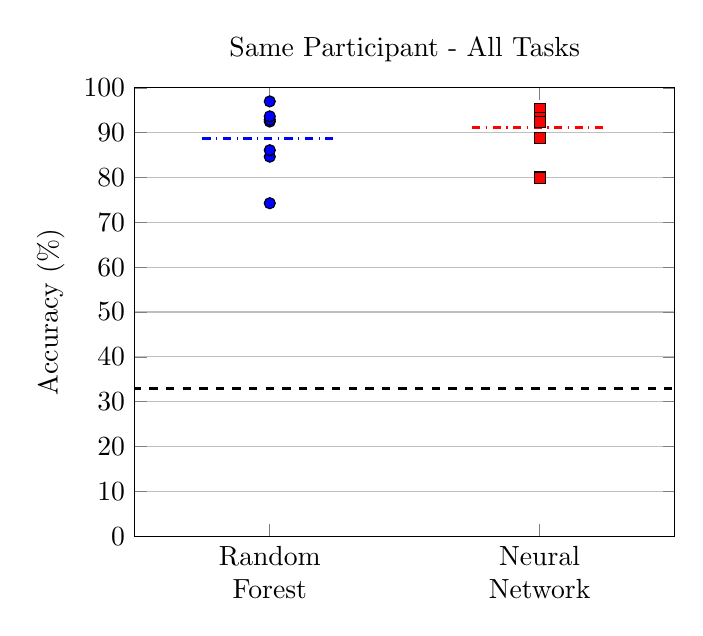
\begin{tikzpicture}
\begin{axis}[
	ymajorgrids,
	scatter/classes= {
		a={mark=*, fill=blue, draw=black},
		b={mark=square*, fill=red, draw=black},
		c={mark=triangle*, fill=brown, draw=black},
		d={mark=diamond*, fill=gray, draw=black}
	},
	ymin=0,
	ymax=100,
	xmin = .5, 
	xmax=2.5,
	ytick={0,10,...,100},
	xtick={1,2},
	xticklabel style={align=center},
	xticklabels={Random\\Forest, Neural\\Network},
	title=Same Participant - All Tasks, 
	ylabel=Accuracy (\%)]

\addplot+[ mark=None, dashed, black, line width = 1pt ]
	coordinates {
	(0, 33)
	(5, 33)	
};

	% Random Forest
	\addplot+[ scatter,
			only marks,
			scatter src=explicit symbolic]
	coordinates {
			(1, 74.27) [a]
			(1, 96.98) [a]
			(1, 84.65) [a]
			(1, 92.49) [a]
			(1, 92.91) [a]
			(1, 93.65) [a]
			(1, 86.10) [a]	
};

% Random Forest Mean
	\addplot+[ mark=None, dashdotted, blue, line width = 1pt ] 
	coordinates {
		(0.75, 88.72)
		(1.25, 88.72)
};

	% ANN
	\addplot+[ scatter,
			only marks,
			scatter src=explicit symbolic]
	coordinates {
			(2, 80.00) [b]
			(2, 95.37) [b]
			(2, 88.88) [b]
			(2, 95.23) [b]
			(2, 93.22) [b]
			(2, 93.23) [b]
			(2, 92.40) [b]
};

% ANN Mean
	\addplot+[ mark=None, dashdotted, red, line width = 1pt ] 
	coordinates {
		(1.75, 91.19)
		(2.25, 91.19)
};


\end{axis}
\end{tikzpicture}

\end{document}
















